\documentclass[runningheads,a4paper]{llncs}
\usepackage{verbatim}
\usepackage{pifont}
\newcommand{\cmark}{\ding{51}}%
\newcommand{\xmark}{\ding{55}}%
\usepackage{makeidx}  % allows for indexgeneration


%\bibliographystyle{splncs}
\usepackage{graphicx}
\title{Accessible EPUB : Making EPUB 3 documents universal accessible}
\titlerunning{Accessible EPUB}
\author{Thorsten Schwarz \and Sachin Rajgopal \and Rainer Stiefelhagen}
\authorrunning{Schwarz et al.} % abbreviated author list (for running head)

\institute{Karlsruhe Institute of Technology, Studycentre for the Visually Impaired, Engesserstr. 4, 76131 Karlsruhe, Germany\\
\email{thorsten.schwarz@kit.edu},\\ WWW home page:
\texttt{http://szs.kit.edu}
}

\begin{document}

\maketitle

\begin{abstract}
Current document standards have the characteristic that they can only serve one group of users under the aspect of vision (sighted, visually impaired or blind reader). Wouldn't it be nice if one documentformat could combine all properties in one document? 
This paper presents a new approach of an universal accessible version of EPUB 3 documents, which will allow sighted, visually impaired and blind readers to use and share the same EPUB 3 document by an "integrated switching mechanism" to change the output format. Furthermore, we will introduce a simple word processing tool that allows to easily create such accessible EPUBs without knowing how an EPUB file is constructed or created. 
\keywords{epub, epub3, accessible documents}
\end{abstract}

\section{Introduction}
In recent years, accessibility has become increasingly important, especially for accessible documents. Several nations have passed regulatory laws that ensure equal treatment of all people and ensure that documents are accessible to all \cite{webaim}.\\
The currently dominant formats for accessible electronic documents are Microsoft Word and PDF (Portable Document Format) documents, or more precisely PDF/UA (PDF/Universal Accessibility) documents. First of all, both formats have a predefined page size. While this is useful for printed documents, a computer screen can rarely display all contents of the document to the detriment of visually impaired people \cite{EPUBzone}. Therefore, an electronic document format - like HTML - without a fixed document size containing semantic and structural information and a fixed reading order would be better suited to meet the requirements of accessibility.\\
Furthermore, different "selectable" forms of presentation would be advantageous, especially for graphics or mathematical formulas. For example, formulas in the \LaTeX source code for blind users or high-contrast images for users with limited residual vision. This could be combined with EPUB 3 \cite{EPUBzone}.

This is exactly where we come in with our new EPUB approach, which combines all three versions in one document. But why is EPUB the format of our choice?

EPUB stands for {\bf E}lectronic {\bf PUB}lication and is a format primarily used for books in an electronic format (E-Book). The EPUB format was created by the International Digital Publishing Forum (IDPF) and the current version is 3.1 which is a minor update to EPUB 3 \cite{EPUBspecs}. EPUB uses XML based formats like XHTML, and thus also uses the accessibility standards and guidelines already established in many nations like the Web Content Accessibility Guidelines (WCAG)\cite{WCAG}. This was done as reading systems can have different screen sizes and the EPUB content can therefore be reflowable. Font type and size can also be adapted to the individual needs of the users. Visually impaired people could therefore adjust the document to their preferences in font style, size and color. The EPUB 3 specification also contains guidelines for accessibility so these features are built in and not an afterthought \cite{EPUB3bp}.

The EPUB working group has also made important changes from EPUB 2 to EPUB 3 which improve the accessibility of documents. For example, mathematical equations can now be displayed in MathML and there is better navigation and more support for Cascading Style Sheets (CSS). However, not all of these changes are yet supported by EPUB readers and devices \cite{EPUB30changes}. 

Creating EPUBs, however, is not as simple as word documents. There are several editors available, but the issues of them will be presented in chapter \ref{ch:exEPUB}. Accessible EPUB is an attempt to remedy these issues and simplify the process so that accessible documents for STEM subjects can be created without intricate knowledge of EPUBs.

\section{Related Work}
Of course, there are already works that have tried to generate different accessible formats. Takaira et al. \cite{unified} created a tool which analyzes a PDF document and outputs different kinds of textbooks by detecting the structure of the document properly assigning the tags.
Leporini et al. \cite{book4all} have created the tool "Book4All" to convert PDF-E-Books into a more accessible format. This was done by analyzing the PDF and converting it into the XML based Intermediate Book Format. This can then be converted into XHTML or Daisy \cite{daisyAccessibility}. 
Coming back to EPUB, Book4All was also developed to create EPUBs and Lenzi and Leporini \cite{voiceover} found out that while there are difficulties using voiceover with EPUBs, this can be improved by using the tags and attributes properly. 
Bartalesi and Leporini \cite{enrichEPUB} carried out an online survey in their work and asked 25 users to rate "enriched" EPUB in comparison to the original PDF format regarding accessibility and usability. $50\%$ of respondents preferred EPUB over other E-Book formats, while $13\%$ said EPUB was equivalent.
The sample group also felt that it was easier to access content in EPUBs and use the table of contents than in PDFs.
Furthermore, $80\%$ of blind users were unable to read images in PDFs correctly with their screen reader, while the corresponding value for EPUBs was less than $50\%$. $64\%$ of users found the EPUB's document structure easy to understand. 

\subsection{Existing EPUB editors}
\label{ch:exEPUB}
There are a number of different ways to create EPUB documents \cite{EPUBprograms}. Adobe InDesign\footnote{https://www.adobe.com/products/indesign.html} is one way and is suitable for publishers, but it has no built-in MathML support and it is a commercial program that is unaffordable to most user groups. LibreOffice in its latest version 6.0 is able to export Writer documents to EPUB, too. This and perhaps Microsoft Word (with installed EPUB macros) are maybe the easiest options to create an EPUB document. Nevertheless, these versions have to be edited in special EPUB editors to meet proper accessiblity levels. For example, alternative texts for images or \LaTeX source code alternatives for mathematical formulas.\\
Some EPUB editors are pure WYSIWYG editors (What You See Is What You Get), but important functions such as mathematical equations and semantic information are usually missing. EPUB editors where the program code has to be edited are limited to persons with programming experience. Sigil \cite{Sigil}, for example, is such a popular open source WYSIWYG EPUB editor with many features, but important features such as text alternatives for images can only be added manually with coding.\\
After all, most editors are not able to produce the kind of universal accessible document we want out of the box, nor accessible to visually impaired or blind people. 

\section{Specifications of our "Accessible EPUB"}

\subsection{EPUB Creation Process}
First of all, what is needed to create an EPUB file and then get it accessible? An EPUB file is nothing more than a ZIP file\footnote{ZIP is an archive file format that supports lossless data compression.} \cite{WhatIsEpub3}, but renamed from "*.zip" to "*.epub". If you change the file extension and extract the file contents, the individual files, such as XHTML and image files, can be opened and edited. The creation of an EPUB document can therefore be briefly described in three steps: 
\begin{enumerate}
\item create content documents (texts, images, etc.) in formats such as XHTML and SVG, 
\item create the package document "package.opf" and 
\item compression of the data including metadata in a ZIP file.
\end{enumerate}
The package document consists of five sections describing how the EPUB document is structured \cite{EPUB3bp}.
\begin{figure}
	\centering
	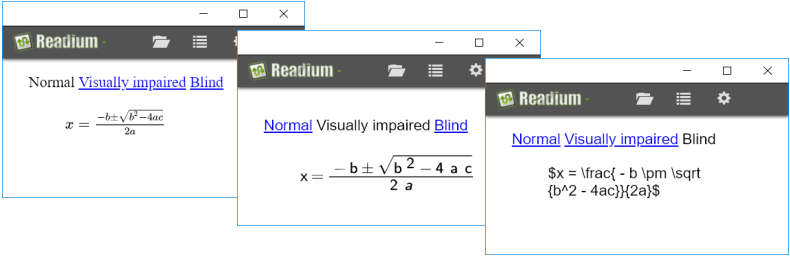
\includegraphics[width=0.95\textwidth]{Equations.png} 
	\caption{EPUB in 'Normal', 'Visual impaired' and 'Blind' mode (from left to right).}
	\label{fig:epub_normal}
\end{figure}

\subsection{EPUB switching mechanism}
The introduction shows that although EPUB 3 is a promising format, the lack of easy-to-use editors means that not everyone can create accessible EPUB documents. Therefore, the main objective of this work is to lay the foundations for such EPUB documents. On the one hand, there is a suitable basic structure that unifies all format versions, and on the other hand, a suitable editor that gets the mentioned problems/restrictions under control for the end user or document creator.\\
This means that, at the end of the day, it should be easy for teachers and other educators to create an EPUB document that can be used by blind, visually impaired and sighted people. By a simple switch in the document, the CSS can be adapted to the needs of the target group with one click (see figure \ref{fig:epub_normal}).\\
For example, the text alternatives for mathematical equations (e. g. the \LaTeX $\mbox{ }$ source code) and images are displayed automatically when the blind version is selected \cite{EPUB3bp}. The switching mechanism can be done either with JavaScript or via CSS. Although JavaScript is easier to use, not all EPUB readers or devices support JavaScript and the EPUB specification does not require JavaScript to be supported \cite{EPUB3bp}. The CSS version is much more limited because all content has to be inserted into a single XHTML file and CSS selectors are not fully supported yet, but CSS support is included in the EPUB specification. Ultimately, we need an EPUB framework that can be used by most end devices, as well as a suitable easy-to-use editor.

Unfortunately a unified accessible standard for the EPUB documents could not be found, as EPUB readers do not support all features mentioned in the EPUB 3 specifications. As a result, Accessible EPUB allows users to create documents either with CSS or JavaScript as basis for the switching mechanism. It is possible that when EPUB readers either have  widespread support for CSS 3 or the specification makes JavaScript support mandatory, one of the standards will establish itself. Until then it is better to design both to allow users to have a choice.
%\begin{figure}
%	\centerline{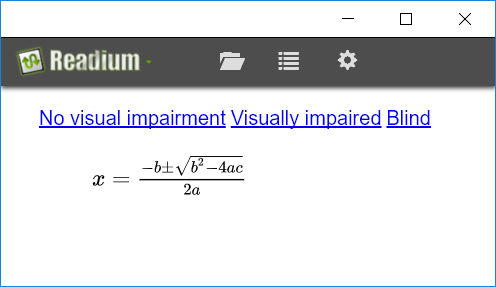
\includegraphics{EquationNormal.png}}
%\end{figure}

%\begin{figure}
%	\centerline{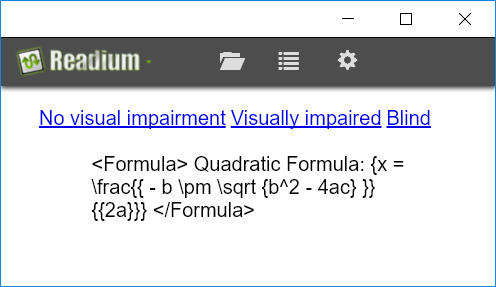
\includegraphics{EquationLatex.png}}
%\end{figure}
%\vspace{-0.6cm} 

%\vspace{-0.6cm} 
\subsection{Editor "Accessible EPUB"}
"Accessible EPUB" is a WYSIWYG program written in C\# (. NET) that serves to create accessible EPUB documents using the switching mechanism (see figure \ref{fig:editor}). The process of creating documents should be as simple as possible so that even people with little experience in using special software can use the program. Primary target groups are, for example, teachers or implementation centers that have a need for accessible documents for different user groups. 

\begin{figure}
	\centering
	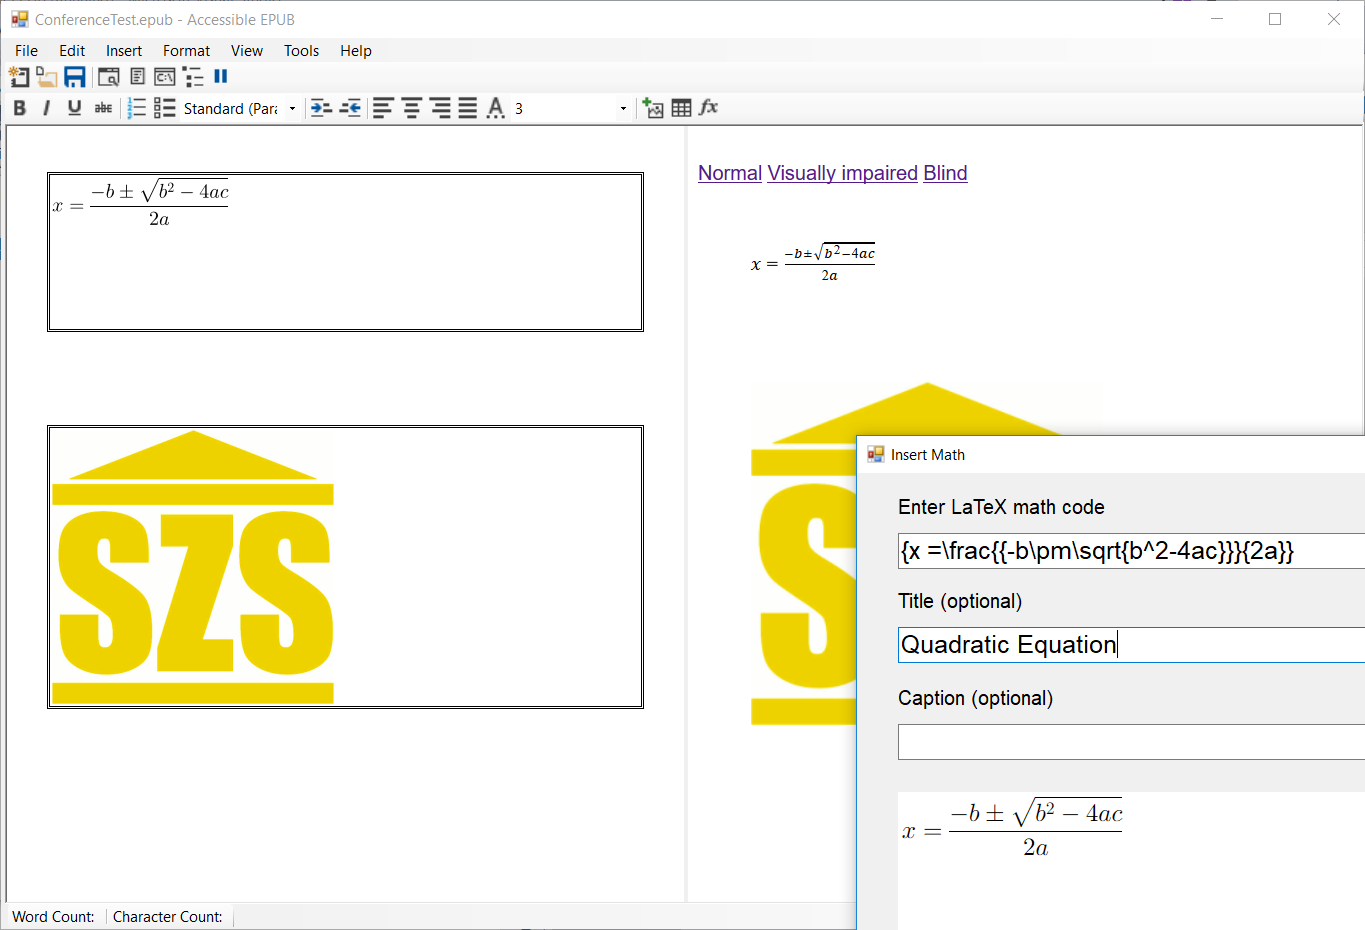
\includegraphics[width=0.9\linewidth]{AccessibleEPUBequationNew.PNG}
	\caption{Accessible EPUB Editor}
	\label{fig:editor}
\end{figure}

A feature is to allow the user to have immediate feedback to their actions. Any text or other content written in the editor on the left side is immediately shown on the right side (figure \ref{fig:editor}). The user can switch between normal, visually impaired and blind versions of the content within the preview browser. 

One of the goals of this project is to create documents for STEM subjects. In other EPUB editors, like Sigil or Adobe InDesign, there is no possibility of adding MathML without coding it in. Equations have to be inserted as normal text or as images. As discussed earlier in this paper, MathML is preferable due to is superior presentation and the ability to interact with equations, such as highlighting a part of an equation. Therefore adding a easy way to insert equations was of particular importance in this program. The equation insertion tool can be seen in figure \ref{fig:editor}. It accepts \LaTeX   code and the result is shown in a panel in the bottom half of the screen. In case of an error, the panel is highlighted with a red border. This immediate feedback should improve the usability of the program.

Tables and images are inserted similarly. When inserting images, the user has to enter some alternative text to ensure the accessibility of the document. Entering a caption and title is optional. All of these will be put in a figure element, and if the user moves it, the caption and alternative text will move it. Editing commands commonly found in word processors are also present in a toolbar at the top of the program.

\noindent Some of the main features of our "Accessible EPUB" editor are: 
\begin{enumerate}
\item It creates an EPUB document with the switching mechanism without having to customize the source code.
\item It includes an equation editor which accepts \LaTeX  as input and inserts the MathML equivalent, SVG image and the alternative text of the equation, as shown in figure \ref{fig:editor}.
\item It provides the ability to insert images with title, caption and alternative text, the last one being mandatory.
\item Is able to insert tables.
\item It gives the possibility to mark up sections using the HTML styles (h1, h2, p, etc.).
\end{enumerate}

\section{Evaluation of the Document Standard}
The document standard was tested on various programs to see if the EPUB can be read properly. The programs tested include Adobe Digital Editions, Calibre, AZARDI and Readium on Windows 10, iBooks under iOS and Reasily under Android. The test examined if they supporte the following: the CSS standard, the JavaScript standard, MathML and screen reader support. The results are shown in table \ref{fig:table}. Several other software readers were tested, like the Bluefire Reader and the Icecream Ebook Reader, but they don't support MathML. Adobe Digital Editions is an exception, but is among the better known readers so it was included in the comparison.
\begin{table}
	\centering
	\caption{Features supported by several EPUB readers}
             \begin{tabular}{| c | c | c | c | c |}
                           \hline
                           & CSS & JavaScript & MathML & Screen reader \\ \hline
                           Adobe Digital Editions & \xmark & \xmark & \xmark & \cmark \\ \hline
                           Calibre & \xmark & \cmark & \cmark & \xmark \\ \hline
                           AZARDI & \xmark & \xmark & \cmark & \cmark \\ \hline
                           Readium & \cmark & \xmark & \cmark & \cmark \\ \hline
                           iBooks & \xmark & \xmark & \cmark & \cmark \\ \hline
                           Bluefire Reader & \xmark & \xmark & \xmark & \xmark \\ \hline
                           Icecream Ebook Reader & \xmark & \xmark & \xmark & \xmark \\ \hline
                           Reasily & \cmark & \xmark & \cmark & \cmark \\ \hline
             \end{tabular}
\label{fig:table}
\end{table}
A first problem was the often missing MathML support. EPUB 3 was approved by the IDPF in 2011, but MathML support is still not common. Even major companies like Adobe do not have MathML support in their Adobe Digital Editions. 
Another point is the support of JavaScript. Only the open source program Calibre supports JavaScript in connection with the storage of sessions, so that the EPUB document retains its appearance until the program is closed. Session and local storages are typically used in web browsers to store personal website settings. A negative aspect of Calibre is that it does not support any screen reader. Another example is Apple's iBooks, which supports JavaScript but does not allow access to the local or session storage. While the inital page changes its style, other pages remain in their default state. Only by leaving iBooks and reopening it, the view is currently adjusted. Reasily for Android supports the same features as Readium and the Android screen reader (Talk Back) works fine. 

CSS 3 support in the form of CSS selectors is also very rare. Only the Windows program Readium supports this and is therefore the only reader that can handle the CSS standard. However, Readium sometimes has problems with selectors that the Gecko-based Mozilla Firefox does not have, for example, so the support can be improved. Readium also supports MathML and screen readers. This makes it the only Windows tool currently available to screen reader users that supports these standards. 
AZARDI is mentioned by the DAISY consortium as an EPUB reader with screen reader support. It shows MathML formulas in the sighted version, but it does not support both CSS and JavaScript switching. Furthermore, a link for switching can be clicked, but it is shown as normal text and not as a hyperlink, so users can’t differentiate between them.

The document standard we created makes extensive use of the new features of EPUB 3, and this is where the problem lies. Even seven years after its approval, support for EPUB 3 is not yet widespread. There is still a lack of suitable readers (on the hardware and software side). The website "EPUB 3 Support Grid\footnote{http://epubtest.org/testsuite/epub3/}" gives a comprehensive overview of which function is supported by which reading system. 

\section{Future Work}
There is still some room for improvement in the compatibility of the EPUB standard, so that it will also be possible to use the documents better with "older" EPUB readers. 
The JavaScript document standard supports multiple HTML files as content documents. If the reader system supports local or session storage, it remembers which version is to be displayed across several HTML files. Accessible EPUB does not yet support this. Adding this feature would allow users to create longer documents and manage individual sections.

Future development will focus on usability and simplified import of other document standards. Currently, users can already import text and HTML documents with certain restrictions so that they can keep their work in these formats. The tool PANDOC can serve as a basis for many formats.
Furthermore, images and formulas will not yet be in the format specified by the document standard during an import, so a wizard will be added that works through each image and formula and allows the user to enter alternative texts.  

Another feature advanced users may want is a source code editor. A code viewer is already available, but currently displays the entire file with the inner workings. The user should not be able to see it, since the processing increases the error possibilities in the document.

We are also considering whether we will start developing suitable readers for various end devices.

\section{Conclusion}
An EPUB document standard has been developed to allow visually impaired, blind and normal-sighted users to use the same document while meeting their respective accessibility requirements. An editor called "Accessible EPUB" was created so that users without programming knowledge can create accessible documents. The document standard uses EPUB 3, which is not yet fully supported by most EPUB reading systems.
It is planned to add features to improve the usability of Accessible EPUB.

\bibliography{icchp}

\bibliographystyle{splncs}

%
% ---- Bibliography ----
%
%\begin{thebibliography}{}
%
%\bibitem[1]{webaim} WebAIM (Web Accessibility in Mind): World Laws: Introduction to Laws Throughout the World, https://webaim.org/articles/laws/world/, visited on 30.01.2018
%\bibitem[2]{EPUBzone} IDPF: Understanding EPUB 3, http://epubzone.org/epub-3-overview/understanding-epub-3, visited on 29.01.2018
%\bibitem[3]{EPUBspecs} IDPF: EPUB 3 Specification, http://www.idpf.org/epub/301/spec/epub-overview.html, visited on 29.01.2018
%\bibitem[4]{WCAG} W3C: Web Content Accessibility Guidelines (WCAG) 2.0, https://www.w3.org/TR/WCAG20/, visited on 29.01.2018
%\bibitem[5]{EPUB3bp} Garrish, M.; Gylling, M.: EPUB 3 Best Practices, 2013, O'Reilly, ISBN 1449329144, 9781449329143
%\bibitem[6]{EPUB30changes} IDPF: EPUB 3 Changes from EPUB 2.0.1, http://www.idpf.org/epub/30/spec/epub30-changes.html, visited on 29.01.2018
%\bibitem[7]{unified} Takaira, T.; Tani, Y.; Fujiyoshi, A.: Development of a Unified Production System for Various Types of Accessible Textbooks, Computers Helping People with Special Needs, 2016, Springer International Publishing, 381-388, ISBN 978-3-319-41264-1
%\bibitem[8]{book4all} Calabr{\`o}, A.; Contini, E.; Leporini, B.: Book4All: A Tool to Make an e-Book More Accessible to Students with Vision/Visual-Impairments, HCI and Usability for e-Inclusion, 2009, Springer Berlin Heidelberg, 236-248, ISBN 978-3-642-10308-7"
%\bibitem[9]{daisyAccessibility} DAISY Consortium: Baseline for Accessible EPUB3, http://www.daisy.org/baseline, visited on 29.01.2018
%\bibitem[10]{voiceover} Bartalesi Lenzi, V.; Leporini, B.: Investigating an Accessible and Usable ePub Book via VoiceOver: A Case Study, Human Factors in Computing and Informatics, 2013, Springer Berlin Heidelberg, 272-283, ISBN 978-3-642-39062-3"
%\bibitem[11]{enrichEPUB} Bartalesi, V.; Leporini, B.: An Enriched ePub eBook for Screen Reader Users, Universal Access in Human-Computer Interaction. Access to Today's Technologies, 2015, Springer International Publishing, 375-386, ISBN 978-3-319-20678-3
%\bibitem[12]{EPUBprograms} DAISY Consortium: Tools for creating EPUB 3 files, http://www.daisy.org/daisypedia/tools-creating-epub-3-files, visited on 29.01.2018
%\bibitem[13]{Sigil} Marković, S.; Schember, J.; Hendricks, K.; Massay, D.: Sigil is a multi-platform EPUB ebook editor, %https://sigil-ebook.com/, visited on 29.01.2018
%\bibitem[14]{WhatIsEpub3} Garrish, M.: What is EPUB 3?, 2011, O'Reilly, ISBN 9781449314545

%\end{thebibliography}

\end{document}